\section{Proofs and Scope of the Mathematical Claims}
\label{app:proofs}
The singular value decomposition $H=U\Sigma V^\top$ separates feature directions from their strengths. For fixed nonnegative weights $w_i$, stacking the scaled source matrices gives
\begin{equation}
 G_S=H_S^\top H_S=\sum_{i\in S}w_iG_i.
 \label{eq:gram}
\end{equation}
The eigenvalues of this sum are the squared singular values of the pooled features. It preserves the strength and cross-pool alignment of directions, provided preprocessing coordinates remain fixed. The experiments use unit weights.

Effective rank normalizes the singular values into a probability vector and exponentiates its entropy \citep{roy2007}:
\begin{equation}
 \reff(H)=\exp\!\left(-\sum_j p_j\log p_j\right),\qquad
 p_j=\frac{\sigma_j(H)}{\sum_k\sigma_k(H)}.
 \label{eq:rank}
\end{equation}
For a nonzero matrix, $0\log0=0$ and $1\leq\reff(H)\leq\operatorname{rank}(H)$, with the upper endpoint attained by equal positive singular values. Two values in ratio $9:1$ give about $1.38$, versus two for equal strengths. Gram eigenvalues must be square-rooted before normalization; normalizing them directly defines another score. Repeating the entire matrix leaves effective rank unchanged: it measures spectral shape, not sample evidence. It is a target-blind comparator, not a step required by the target-aware scores.

For fixed $H_S$ and Gaussian likelihood, completing the square in the prior times likelihood gives posterior precision $P_0^{-1}+\sigma^{-2}H_S^\top H_S$ and mean $\mu_S=P_S\sigma^{-2}H_S^\top y_S$. For an independent target observation $y=h^\top\theta+\epsilon$, conditional on the training data and $h$,
\begin{equation}
 \E[(y-h^\top\mu_S)^2\mid H_S,y_S,h]=\sigma^2+h^\top P_Sh.
\end{equation}
Integrating $h$ gives Equation~\eqref{eq:risk}. We assume the target covariate distribution does not reveal additional information about $\theta$ beyond this model. If a source has a different regression function, or labels are multiclass with softmax readout, this derivation no longer identifies the evaluated loss. The proof does not bound this misspecification error. Replacing $C_T$ by a finite-sample estimate adds another discrepancy not removed by the identity.

Let $S_Q$ minimize $\ell$ over $\cQ_s$. Uniform deviation on that shortlist gives
\begin{equation}
 \ell(\widehat S)\leq v(\widehat S)+\varepsilon
 \leq v(S_Q)+\varepsilon\leq\ell(S_Q)+2\varepsilon.
\end{equation}
Subtracting $\min_{S\in\cC}\ell(S)$ proves Equation~\eqref{eq:decomposition}. No probability is asserted by this algebra. For population generalization, one must additionally justify the deviation event using the actual dependence and selection scheme. Exhaustive finite-test scores alone do not supply that justification.

The feature map $\phi(h)=hh^\top$, equipped with Frobenius inner product, satisfies $\langle\phi(h),\phi(h')\rangle_F=(h^\top h')^2$. The squared distance between source and target empirical feature means is therefore Equation~\eqref{eq:mmd}. This is the biased empirical squared MMD (a V-statistic), not the diagonal-excluded unbiased estimator. It depends on uncentered second moments and cannot distinguish all distributions sharing those moments. We use it as a computationally simple same-information comparator, not a complete discrepancy measure.

\subsection{Equal-cost reversal of moment matching and target risk}
\label{app:equal-cost-reversal}
Take unit basis vectors $e_1,e_2$ and a target distribution assigning them probabilities $3/4$ and $1/4$. Use a common four-row source block with counts $(3,1)$ of the two basis vectors, and two alternative four-row blocks with counts $(3,1)$ and $(2,2)$. Combining the common block with either alternative gives $G_A=\operatorname{diag}(6,2)$ or $G_B=\operatorname{diag}(5,3)$, each with eight samples and trace eight. Then $G_A/8=C_T$ and $G_B/8-C_T=\operatorname{diag}(-1/8,1/8)$, giving squared MMD $0$ and $1/32$. Under the shared Gaussian linear model with unit prior precision and observation noise variance, the two posterior covariance matrices are $\operatorname{diag}(1/7,1/3)$ and $\operatorname{diag}(1/6,1/4)$. Weighting by $C_T$ yields $4/21$ and $3/16$, respectively. The common irreducible noise cancels, so the predictive risk of $A$ exceeds that of $B$ by $1/336$.

\section{Implementation and Audit Details}
\label{app:protocol}
The original DomainNet study fits a ridge readout and transforms its scores into class probabilities. Its weights and Brier loss are
\begin{equation}
 \begin{aligned}
 W_S&=(I+G_S)^{-1}\sum_{i\in S}H_i^\top Y_i,\qquad
 p(x)=\operatorname{softmax}(h(x)^\top W_S),\\
 b(S)&=\frac1{n_T}\sum_t\norm{p(x_t)-e_{y_t}}_2^2.
 \end{aligned}
\end{equation}
$Y_i$ is the one-hot source-label matrix over the fixed 100-class vocabulary. There is no intercept or temperature tuning. Linear algebra uses float64 after loading float32 features. For effective rank obtained through a Gram eigendecomposition, negative roundoff eigenvalues are clipped to zero, square roots form singular values, and only $\sigma_j>\sigma_{\max}\sqrt{8\epsilon_{64}\max(n_S,d,1)}$ are retained. The zero matrix returns rank zero in code. This tolerance concerns numerical rank; the entropy definition itself is unchanged. The shared projection uses seed $20260911$ and $d=128$; no outcome-dependent dimension choice is used within the frozen DomainNet protocol.

Bayesian D-opt maximizes $\log\det(I+G_S)$. Subspace DPP takes each block's top 16 Gram eigenvectors $U_i$, defines $K_{ij}=\norm{U_i^\top U_j}_F^2/16$ with $K_{ii}=1$, numerically projects the matrix to a PSD correlation matrix, and maximizes $\log\det(K_{S,S}+10^{-8}I)$. Its kernel describes block subspaces, not individual-image features. Domain balance maximizes the number of represented domains minus $10^{-3}$ times the sum of squared domain block counts. Deterministic scores break ties lexicographically by combination identifier. These choices are fixed comparators; poor performance of this DPP construction is not a result about all determinantal selection methods.

DomainNet records image content hashes, sample identifiers, official split membership, role assignments, and class vocabulary. Archive and split checksums are validated before feature extraction. Disjoint role membership and duplicate-content checks address overlap within the materialized benchmark; they do not rule out semantic near-duplicates or pretraining contamination. All screen methods use the same source blocks, projection, target-selection rows, and candidate family. Feature extraction ignores labels, while benchmark materialization uses taxonomy metadata and stores labels for later authorized stages.

Screen, validation, and audit manifests bind configuration and upstream artifact hashes. Stage-specific loaders enforce label and split permissions. In the original protocol, validation evaluates each method or random repeat separately. The test audit covers all $6\times455$ combinations per encoder after choices are frozen; its exhaustive oracle serves as a research reference. The follow-up caching policy is described below.

Seeds $20260917$, $20260918$, $20260919$, and $20260920$ generate new 128-dimensional Rademacher projections with the same pre/post row normalization. Seed $20260911$ is an implementation control, excluded from new-seed means. Logistic regression uses L2 regularization, $C=1$, no intercept, LBFGS, tolerance $10^{-6}$, and at most 1,000 iterations. A convergence warning aborts a task; no such warning occurred, and the largest iteration count was 24. The class vocabulary is fixed, with zero probability assigned to source-absent classes.

All methods retain their screening rules, candidate combinations, and five shortlist sizes. Separate processes screen, fit and validate, then test frozen models. The audit checks source, configuration, lineage, model, and selection hashes before reading test features. The follow-up fits every combination once per readout and reuses these fits across methods. This cached exhaustive evaluation supports counterfactual comparisons of shortlists. Brier, NLL, and error use their own validation losses for final selection. Original-seed ridge reproduces 5,460 reconstructed test combinations with maximum loss difference $1.78\times10^{-15}$ and all 1,620 Brier validation choices exactly.

The two encoders and five seeds produce 54,600 fits across both readouts. New-seed summaries first average random repeats within a task, then encoders and seeds within each target domain, and finally the six domains. Each readout contributes 48 repeated encoder--seed--domain measurements. They remain six domain units sharing the same source pools.

The anonymous code archive records image and feature hashes and provides outcome tables. The DomainNet configuration is \path{code/configs/target_conditioned_e2b/domainnet_v1.json}; its experiment is in \path{results/target_conditioned/e2b_fixed_cost_shortlist/domainnet_v1/}. The projection and readout archive is in \path{results/target_conditioned/revision_20260917/}. The fixed-cost budget, construction and timing records are in \path{results/target_conditioned/revision_20260922/}.

\begin{algorithm}[htbp]
\caption{Target A-opt screening and validation}
\label{alg:target-a}
\begin{algorithmic}[1]
\Require Source pools $\{D_i\}$, candidate family $\cC$, target sets $T_{\rm sel},T_{\rm val}$.
\Require Fixed feature map $h$, fitting rule $\mathcal A$, loss $L$, shortlist size $1\leq s\leq|\cC|$.
\Ensure Shortlist $\cQ_s$, selected combination $\widehat S$, and fitted readout $q_{\widehat S}$.
\State Form $H_i$ and $H_{\rm sel}$ using $h$, without reading labels.
\State Cache $G_i=H_i^\top H_i$; estimate $\widehat C_T=H_{\rm sel}^\top H_{\rm sel}/|T_{\rm sel}|$.
\For{each $S\in\cC$}
  \State $G_S\gets\sum_{i\in S}G_i$; $f_A(S)\gets\tr\!\left[\widehat C_T(I+G_S)^{-1}\right]$.
\EndFor
\State Retain the first $s$ candidates ordered by $(f_A(S),\operatorname{id}(S))$ as $\cQ_s$.
\For{each $S\in\cQ_s$}
  \State Fit $q_S\gets\mathcal A(H_S,y_S)$ using source labels.
  \State $v(S)\gets |T_{\rm val}|^{-1}\sum_{(x,y)\in T_{\rm val}}L(q_S(h(x)),y)$.
\EndFor
\State Choose $\widehat S$ minimizing $(v(S),\operatorname{id}(S))$ over $\cQ_s$.
\State \Return $\cQ_s,\widehat S,q_{\widehat S}$.
\end{algorithmic}
\end{algorithm}

\subsection{Static-screen checks}
\label{app:diagnostics}
Table~\ref{app:construction-table} compares hash repartitioning with the original pools at fixed projection and sample cost. Each domain's same 1,536 images are deterministically hashed into three blocks; target data roles stay fixed. Domain matching uses source-domain rather than block moments and creates composition ties. The post-hoc randomized comparator averages 20 frozen tie orders. When retaining half of each non-singleton composition stratum, domain-only matching has exact expected optimum retention of $45.68\%$ under uniform ties. Figure~\ref{fig:recall} shows recall across budgets.

At $K=3$ on PACS/Office-Home, mean Brier is $0.826769$ for Target A-opt, $0.829162$ for DPP and $0.828719$ for MMD. Paired intervals for the Target A-opt minus baseline difference are $[-0.007449,0.000731]$ and $[-0.003392,-0.000712]$, respectively. The post-hoc audit covers 220 combinations per task. For the archived DomainNet projections, the lowest Target A-opt classification-error recall occurs on DINOv2/Quickdraw with logistic regression and seed $20260918$; the shortlist still contains the test-error oracle.

For the static timing in Section~\ref{sec:cost}, methods start with resident projected features and independently rank, fit and validate in three runs per encoder, target and readout. Measured image accounting adds initialization, I/O, extraction and projection. Candidate construction and test auditing sit outside the timing.

\begin{figure}[t]
\centering
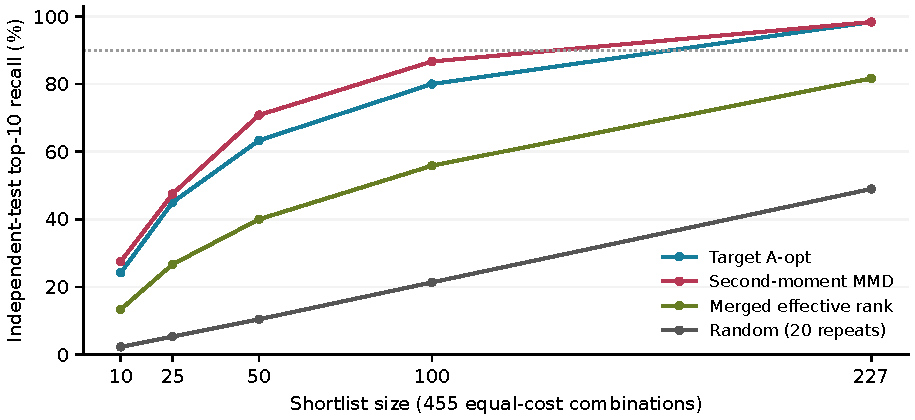
\includegraphics[width=\linewidth]{shortlist_recall.pdf}
\caption{Mean test Brier top-ten recall is shown across shortlist sizes in the original DomainNet study. The dotted line marks the prespecified recall threshold. All curves use the same candidate combinations and feature access appropriate to each rule.}
\label{fig:recall}
\end{figure}

\begin{table}[ht]
\centering
\caption{The construction challenge uses logistic Brier. Final loss is validation-selected at $s=50$. The last columns measure retention of one empirical optimum when half of each non-singleton domain-composition stratum is kept, not final selection accuracy. Means average strata and encoders within targets, then six targets. Domain matching uses 20 randomized tie orders for final loss; its within-stratum entry is the exact uniform-tie expectation.}
\label{app:construction-table}
\begin{tabular}{lrrrr}
\toprule
 & \multicolumn{2}{c}{Final Brier ($s=50$)} & \multicolumn{2}{c}{Within-composition (\%)}\\
Screen & Original & Hash & Original & Hash\\
\midrule
Target A-opt & 0.863170 & 0.869699 & 77.22 & 55.83 \\
MMD & 0.863110 & 0.869257 & 76.11 & 55.00 \\
Mean matching & 0.863713 & 0.873038 & 75.28 & 57.78 \\
Domain moment (random ties) & 0.863667 & 0.869356 & 45.68 & 45.68 \\
Random & 0.870013 & 0.874244 & 45.04 & 45.31 \\
\bottomrule
\end{tabular}

\end{table}

\section{Sequential pool querying}
\label{app:pool-query}

\begin{proposition}[Identification under exact additivity]
\label{prop:pool-identification}
For the complete family of triples from 15 pools, suppose $v(S)=x_S^\top\beta$ for every candidate $S$ and a query reveals $v(S)$ exactly. The 15 scores from any full-rank set of 15 query rows determine every validation score in the family.
\end{proposition}
\begin{proof}
Each pool occurs in $\binom{14}{2}=91$ triples, and each pair occurs in $\binom{13}{1}=13$ triples. Hence the full incidence matrix satisfies $X^\top X=78I+13\mathbf{1}\mathbf{1}^\top\succ0$. A full-rank queried design $X_Q$ gives the unique coefficient vector $X_Q^{-1}v_Q$. Multiplying by $X$ gives the entire loss vector. A separate intercept is redundant because $x_S^\top\mathbf{1}=3$ throughout the family. With fewer than 15 queries, a nonzero direction in the nullspace of $X_Q$ leaves the queried values fixed and changes at least one unqueried value. Thus fewer queries cannot identify the full table in general, even for adaptive queries. One can take an arbitrarily small perturbation about the constant loss vector with all entries equal to one to keep both tables in the Brier range.
\end{proof}

This proposition concerns the measured validation-loss surface for a fixed fitting and validation protocol. Real losses can depart from additivity, and the coefficients are working-model parameters. Obtaining a fitted readout for an unqueried minimizer requires one further query. Algorithm~\ref{alg:pool-query} can instead allocate its next query to exploration and returns the best observed candidate. Its leverage term is a heuristic with no confidence calibration.

\begin{algorithm}[H]
\caption{Pool querying with validation feedback}
\label{alg:pool-query}
\begin{algorithmic}[1]
\Require Candidate incidence matrix $X$ of rank $p$, budget $p\leq B\leq|\cC|$, query mode, and a fit-and-validate query.
\State Select $p$ rows by greedy pivoted Gram--Schmidt on $X$.
\State Fit and validate those candidates to initialize $Q$ and $v_Q$.
\While{$|Q|<B$}
  \State Fit $\widehat\beta\gets\arg\min_\beta\|v_Q-X_Q\beta\|_2^2$.
  \State Rank unqueried candidates by increasing score in Equation~\eqref{eq:pool-acquisition}.
  \State Take the first candidate (sequential) or the first $B-|Q|$ candidates (two-batch).
  \State Fit and validate those candidates and append their rows and losses to $Q$ and $v_Q$.
\EndWhile
\State \Return the queried candidate minimizing $(v(S),\operatorname{id}(S))$ and its fitted readout.
\end{algorithmic}
\end{algorithm}

Initialization repeatedly projects each unchosen row onto the span of the selected rows and chooses the row with the largest squared residual. We round the squared residuals and query scores to 12 decimal places and break ties by lexicographic candidate ID. For 15 pools labeled $A$ through $O$, each row starts with squared norm $3$, so $\mathrm{ABC}$ comes first. After that pivot, $\mathrm{ABD}$ has squared residual $3-2^2/3=5/3$, whereas $\mathrm{DEF}$ retains squared norm $3$. The full order is
\[
\begin{gathered}
 \mathrm{ABC,\ DEF,\ GHI,\ JKL,\ MNO,\ ADG,\ AEH,\ AFI,}\\
 \mathrm{BJM,\ BKN,\ BLO,\ DEI,\ DHJ,\ DKM,\ JKO}.
\end{gathered}
\]
The first five triples cover all pools but provide only five independent sums. The remaining pivots add ten independent directions. Full column rank makes $X_Q^\top X_Q$ invertible, and adding queried rows preserves that rank. Query budgets 15, 25 and 50 use nested prefixes. The geometry-offset ablation uses the same initialization and query rule, fitting least squares to $v(S)-g(S)$ and adding $g(S)$ to the predicted score. With $N=455$ candidates and zero-based ranks, $g(S)=0.005[\operatorname{rank}_A(S)+\operatorname{rank}_M(S)]/[2(N-1)]$. The pool-only rule sets $g(S)=0$ throughout.

In the archived replay, we lock the query trajectories before test auditing. The four additional projections reuse losses of fitted models on six targets and two encoders. Mean test Brier is $0.864174$ for sequential 25, $0.864365$ for fixed MMD 50 and $0.864118$ for full validation. The 24 paired seed--domain means stay within $+0.005$ of both references. At 25 fits, the geometry-offset ablation changes two of 48 winners and increases mean Brier by $0.000007$.

\section{Calibration and transport under fixed candidate membership}
\label{app:calibration-transport}
Both checks use the original DomainNet pool membership, six target domains, two encoders, and projection seed 20260911. We average random orders within each domain and encoder, then average encoders within each domain and weight the six domains equally. Each quality gap subtracts the corresponding 455-fit validation winner's test Brier.

\subsection{Ridge temperature calibration}
\label{app:ridge-temperature}
We retain ridge regularization $\lambda=1$. Reconstructing the $T=1$ scores across all candidates gives maximum Brier discrepancies of $1.95\times10^{-9}$ on validation and $1.86\times10^{-9}$ on test across the 12 units. We use the test comparison only to check reconstruction. For candidate scores $z$, we evaluate $\operatorname{softmax}(z/T)$ and choose $T$ by minimum validation Brier on a fixed grid of 81 log-spaced values from $0.01$ to $100$.

First, we fix the original full-validation winner in each unit and fit its temperature on all 1,024 validation examples. Mean test Brier changes from $0.986695$ to $0.743338$, with the same $36.00\%$ top-1 accuracy. The uniform-probability reference is $1-1/100=0.99$. Second, we split validation by a fixed sample-ID hash. We fit each candidate's temperature on 512 examples and select a candidate on the other 512. We freeze temperatures and winners before final test evaluation. Table~\ref{tab:ridge-calibration} reports this reselection arm. At 227 fits, both geometric screens recover the calibrated full-validation winner in all 12 units. The calibration study fixes the feature dimension and ridge regularization. Appendix~\ref{app:server-timing} measures the cost of this split-validation protocol.

\begin{table}[ht]
\centering
\caption{Ridge results after temperature fitting and reselection on disjoint halves of validation. The last column counts domains whose signed mean test Brier gap to calibrated full validation exceeds $+0.005$.}
\label{tab:ridge-calibration}
\begin{tabular}{rlrrrr}
\toprule
Fits & Screen & Test Brier & Top-1 & Brier gap & Domains \\
\midrule
50 & Target A-opt & 0.725347 & 37.63\% & $-0.000150$ & 1/6 \\
50 & MMD          & 0.727958 & 37.61\% & $+0.002461$ & 2/6 \\
50 & Random       & 0.742038 & 36.35\% & $+0.016541$ & 5/6 \\
227 & Target A-opt & 0.725498 & 37.78\% & $+0.000000$ & 0/6 \\
227 & MMD          & 0.725498 & 37.78\% & $+0.000000$ & 0/6 \\
227 & Random       & 0.730224 & 37.37\% & $+0.004726$ & 2/6 \\
455 & Full validation & 0.725498 & 37.78\% & $+0.000000$ & 0/6 \\
\bottomrule
\end{tabular}
\end{table}

\subsection{Sliced Wasserstein on the same candidates}
\label{app:transport-fixed}
We score the 455 fixed unions using the same frozen source and unlabeled target screening features as the geometric screens. For each of 32 fixed Gaussian unit directions, we sort the projected values of the 1,536 candidate and 1,536 target examples and compute the mean squared difference between corresponding sorted values. We average those distances. The whitened variant applies an inverse square root of the pooled, centered source covariance with ridge $0.1$ times the mean eigenvalue. It uses one transform per encoder and target, shared across candidates. The comparison tests transport-based alignment under the fixed-pool protocol. TAROT \citep{feng2025tarot} uses supervised loss-gradient features and sample-level selection.

We verify that recalculated Target A-opt and MMD match all top-50 and top-227 sets in the paired readout archive. We freeze rankings before using archived logistic validation loss to select winners and test loss to audit them. Table~\ref{tab:fixed-transport} reports timings for ranking only. Each unit uses the median of three single-thread runs from resident projected features, including whitening when applicable, and the reported times average units. Section~\ref{sec:cost} reports a separate static-screen timing study that includes fitting and validation and accounts for feature extraction. At 227 fits, the absolute mean gap to full validation is below $0.0005$ for all four geometric screens.

\begin{table}[ht]
\centering
\caption{Fixed-pool transport comparison with logistic readouts at 50 fits. Gaps are relative to full validation over 455 candidates. Seconds cover ranking from resident projected features.}
\label{tab:fixed-transport}
\begin{tabular}{lrrrr}
\toprule
Screen & Test Brier & Brier gap & Seconds & Domains $>+0.005$ \\
\midrule
Sliced Wasserstein & 0.866406 & $+0.002649$ & 0.2777 & 1/6 \\
Whitened sliced Wasserstein & 0.865342 & $+0.001585$ & 0.2948 & 0/6 \\
Target A-opt & 0.864104 & $+0.000347$ & 0.5482 & 0/6 \\
MMD & 0.863951 & $+0.000194$ & 0.0387 & 0/6 \\
Random & 0.871557 & $+0.007800$ & \textemdash & 4/6 \\
Full validation & 0.863757 & $+0.000000$ & \textemdash & 0/6 \\
\bottomrule
\end{tabular}
\end{table}

\subsection{Inverse weighting and calibrated ridge time}
\label{app:server-timing}
At 50 fits on the same DomainNet logistic candidates, Target A-opt gives mean test Brier $0.864104$, compared with $0.896467$ for linear target energy, which omits inverse weighting, and $0.863951$ for MMD.

We separately time the split-validation ridge protocol with $\lambda=1$ from resident projected features and precomputed rankings. The interval includes block statistics, fitting, temperature search and choosing a winner. Target A-opt 50 and MMD 50 each take $1.114$ s versus $10.047$ s for full validation, averaging three-run medians across 12 encoder--domain units. Temperature search takes about $93$--$94\%$ of calibrated time.

\section{Fresh evaluations and linear-design comparisons}
\label{app:fresh-eval}

\subsection{Benchmarks and locked selection}
\label{app:fresh-protocol}
We ran a new campaign with freshly obtained data and supervised fits. The cleaned DomainNet split contributes 100 of its 345 classes, chosen by a fixed hash before training. Each of the six domains provides 1,536 source images, 512 unlabeled target-screen images and 1,024 target-validation images from disjoint roles in the official training split. We reserve 2,048 test images per domain from the official test split. For each target, the other five domains each supply three pools of 512 images. Each candidate trains on three pools (1,536 images). We extract frozen ImageNet-pretrained ResNet-50 features and use 128-dimensional random projections with row normalization before and after projection. Four seeds vary the projection and hash-based pooling. Within each source domain, the second construction sorts images along the first principal component of the centered source features (PC1) and cuts equally sized pools. Both constructions use the same image inventory.

For Optdigits \citep{alpaydin1998optdigits}, each seed takes 3,000 official training examples and constructs 15 artificial pools of 200 examples by hash or source-feature PC1. The official test split uses different writers. We divide it by sample-ID hash into 256 unlabeled screening examples, 512 validation examples and 1,029 held-out test examples. The readout inputs are the native 64-dimensional count features, scaled by $1/16$ and row-normalized. We use the same four seeds and score all eight seed--construction configurations.

Both benchmarks use multinomial logistic regression with $C=1$, no intercept, and an L-BFGS tolerance of $10^{-6}$ with a cap of 1,000 iterations. We align predictions to a fixed label vocabulary and assign zero probability to absent training classes. Before any test evaluation we lock the candidate choices. Every policy can use only its queried validation losses, and the 455-fit reference is the validation winner. The same winner is scored by test Brier, top-1 accuracy and negative log likelihood (NLL), with a probability floor of $10^{-15}$ for NLL. On DomainNet/PC1, sequential 25 improves mean test Brier over MMD 25 ($0.909862$ versus $0.913940$), while its NLL is higher ($4.011643$ versus $3.858980$). All seeds share the original datasets. The $+0.005$ threshold describes individual configuration gaps to full validation. Random policies average 20 frozen orders within each configuration.

\subsubsection{Diagnosing the additive approximation}
For Optdigits, fitting all 455 validation scores gives additive $R^2$ of $0.851$ for hash and $0.169$ for PC1. After 25 queries, prediction $R^2$ on still-unqueried candidates is $0.637$ for hash and $-7.57$ for PC1. These diagnostics read scores unavailable during selection. A deployment check would require held-out queries charged to the budget because 15 independent rows can interpolate the first 15 scores.

\subsection{Linear best-arm identification and experimental design}
\label{app:fresh-linear}
An arm here is a pool combination and its known feature is the 15-dimensional pool incidence vector. The negative validation loss plays the role of an arm reward. Linear best-arm identification and transductive design already use shared features to infer which candidate is best \citep{soare2014linbai,fiez2019transductive}. In our fixed validation task, a repeated evaluation supplies the same score. Pool interactions may cause systematic departures from the linear model. In particular, the $0.001$ exploration coefficient is a heuristic in this setting.

The follow-up compares policies on the same 48 DomainNet and eight Optdigits configurations, using a reveal-only replay of validation scores from the fresh fits. It uses a previously inspected benchmark with the new comparison protocol fixed before the new baseline outcomes. All incidence-based methods start with the same 15 independent rows and use ordinary least squares on queried scores. We count distinct candidate fits and use 25 as the primary budget, with 50 and 100 as checks. Let $V$ be the Gram matrix of the queried incidence rows. For a possible next row $x$, the greedy D-design maximizes $x^\top V^{-1}x$. A-design minimizes the trace of the inverse updated Gram matrix. G-design minimizes the maximum predictive variance over candidate rows, and XY-design minimizes the maximum variance of any pairwise candidate difference. These are one-step designs for the incidence model. Target A-opt uses a separate target-weighted criterion on the classifier features. Our finite-budget LinGapE adaptation \citep{xu2018lingape} identifies a predicted incumbent and a challenger based on the predicted gap and its uncertainty, then queries an unused row that minimizes the uncertainty of that gap. It uses the shared 15-row initialization and four fixed scaling coefficients, $0.001$, $0.01$, $0.1$ and $1$.

All adapted baselines can use $B-1$ policy queries plus one fit of the best predicted unqueried candidate, then return the lowest validation loss among the $B$ fits. Checks also evaluate spending all $B$ fits on the policy and returning the best observed model, or returning the $B-1$-fit prediction once its model is available. All choices lock before test auditing. On DomainNet/PC1, reserving the fit reduces D-design's mean test gap to full validation from about $0.0128$ to $0.0010$. On Optdigits/PC1, XY-design reduces mean validation regret, the gap to the minimum validation loss, from $0.059715$ (sequential 25) to $0.009403$. Table~\ref{tab:fresh-linear-breakdown} reports the matched budget by construction. Original OD-LinBAI requires a larger nominal budget in this setting \citep{yangtan2022linbai}. At 41--43 distinct fits its relative performance depends on partition and termination rule.

\begin{table}[!htb]
\centering
\caption{Test Brier by dataset and pool construction in the linear-design comparison. All low-budget rows use 25 candidate fits. D/A/G/XY and the LinGapE adaptations reserve one fit to instantiate a prediction. Pool-query ablations, MMD and Target A-opt select the best validation score among their queried candidates.}
\label{tab:fresh-linear-breakdown}
\begin{tabular}{lrrrr}
\toprule
 & \multicolumn{2}{c}{DomainNet} & \multicolumn{2}{c}{Optdigits} \\
\cmidrule(lr){2-3}\cmidrule(lr){4-5}
Policy & Hash & PC1 & Hash & PC1 \\
\midrule
Sequential & 0.922283 & 0.909862 & 0.299730 & 0.406669 \\
Two-batch & 0.922263 & 0.909912 & 0.300364 & 0.406669 \\
Pure exploitation & 0.922283 & 0.909940 & 0.299730 & 0.406669 \\
D-design & 0.922524 & 0.910907 & 0.300751 & 0.406229 \\
A-design & 0.922502 & 0.911131 & 0.302644 & 0.376545 \\
G-design & 0.922509 & 0.911892 & 0.300364 & 0.371922 \\
XY-design & 0.922463 & 0.912276 & 0.301795 & 0.345173 \\
LinGapE adaptation, $c=0.001$ & 0.922291 & 0.911066 & 0.302299 & 0.403567 \\
LinGapE adaptation, $c=0.01$ & 0.922551 & 0.910722 & 0.301396 & 0.403567 \\
LinGapE adaptation, $c=0.1$ & 0.922711 & 0.910773 & 0.301733 & 0.406669 \\
LinGapE adaptation, $c=1$ & 0.922634 & 0.910854 & 0.301726 & 0.380168 \\
MMD & 0.926531 & 0.913940 & 0.302909 & 0.339867 \\
Target A-opt & 0.922727 & 0.911755 & 0.304332 & 0.339867 \\
Full validation (455 fits) & 0.922216 & 0.909941 & 0.299730 & 0.339867 \\
\bottomrule
\end{tabular}
\end{table}

\subsection{Independent logistic timing}
\label{app:fresh-timing}
Resident-feature timing separately reruns ranking or query calculation, fitting and validation. DomainNet uses six targets, hash pools and the first seed; Optdigits uses the first hash seed. Each strategy has three rotated repeats per configuration, with one BLAS thread per fitting worker. Cache decoding, integrity checks and test scoring sit outside decision time.

\begin{table}[!htb]
\centering
\caption{Logistic decision time in seconds from resident features, with one and four fitting workers. DomainNet entries are medians of 18 runs and Optdigits entries are medians of three runs.}
\label{tab:fresh-logistic-time}
\begin{tabular}{lrrrr}
\toprule
 & \multicolumn{2}{c}{DomainNet} & \multicolumn{2}{c}{Optdigits} \\
\cmidrule(lr){2-3}\cmidrule(lr){4-5}
Policy & One & Four & One & Four \\
\midrule
Sequential 25 & 3.337 & 1.922 & 0.552 & 0.642 \\
Two-batch 25 & 3.284 & 1.154 & 0.526 & 0.762 \\
MMD 25 & 3.168 & 1.107 & 0.550 & 0.897 \\
MMD 50 & 6.228 & 2.069 & 1.092 & 1.630 \\
Target A-opt 25 & 3.223 & 1.347 & 0.614 & 0.867 \\
Full validation & 59.585 & 19.243 & 9.632 & 12.223 \\
\bottomrule
\end{tabular}
\end{table}

We also time the complete pipeline from locally available images and pretrained weights on a V100 for the preselected Clipart/hash configuration. Each policy starts without extracted features, runs once with one fitting worker, and pays for model loading, image I/O and transforms, extraction, projection and decision. The sequential and two-batch policies and full validation each encode 8,704 images. MMD encodes a further 512 unlabeled target-screen images. The total seconds are $19.602$ (sequential 25), $19.646$ (two-batch 25), $23.885$ (MMD 50) and $76.480$ (full validation). Downloads, Python import time and forced eviction of the OS cache fall outside this timing. The single run per method gives a Clipart case study.

\subsection{Ridge calibration and feature-dimension sensitivity}
\label{app:fresh-ridge}

We use the first DomainNet hash seed with five nested projections. Calibration uses the first validation half to choose temperature over 81 log-spaced values from $0.01$ to $100$. The tuned arm jointly chooses $\lambda\in\{0.1,1,10\}$ and uses three supervised fits per candidate. All arms choose the winning candidate on the second half and share the geometric rankings. Table~\ref{tab:fresh-ridge-sensitivity} compares calibrated methods under matching settings.

\begin{table}[htbp]
\centering
\caption{Fresh DomainNet ridge sensitivity, hash pools and first seed. Brier uses equal weighting across six domains. Each count gives the number of domains for which sequential 25 has a signed test Brier gap above $+0.005$ relative to full validation with that column's calibration and regularization.}
\label{tab:fresh-ridge-sensitivity}
\begin{tabular}{r rrr rrr}
\toprule
 & \multicolumn{3}{c}{Calibrated, fixed $\lambda$} & \multicolumn{3}{c}{Calibrated, tuned $\lambda$} \\
\cmidrule(lr){2-4}\cmidrule(lr){5-7}
Dimension & Seq.\ 25 & Full & Count & Seq.\ 25 & Full & Count \\
\midrule
64  & 0.880595 & 0.878260 & 2/6 & 0.880624 & 0.877666 & 2/6 \\
96  & 0.846247 & 0.844187 & 2/6 & 0.844467 & 0.843555 & 1/6 \\
128 & 0.827308 & 0.827477 & 0/6 & 0.830918 & 0.827681 & 1/6 \\
256 & 0.785407 & 0.780673 & 3/6 & 0.779687 & 0.776171 & 2/6 \\
512 & 0.752150 & 0.753835 & 1/6 & 0.745405 & 0.749862 & 1/6 \\
\bottomrule
\end{tabular}
\end{table}

\subsection{Exploratory scale and budget checks}
The constructed Clipart ranking stress test yields identical exact Target A-opt top-50 lists at 4,060 candidates, taking $1.23$ s versus $2.35$ s for exhaustive scoring. A retrospective leave-one-domain MMD stopping rule uses $47.92$ rather than 50 fits on average, with no domain-mean test gap above $+0.005$ for either policy. A-opt and random use more fits with this stopping rule. These are static ranking and single-projection stopping checks. The pool-query results use a fixed budget and 455 candidates.
